\mysubsection{Sarah Häfele}{Erste Ideen}

Nach der ersten Phase des ungeordneten Brainstormings zeichnen sich zwei verschiedene Spielideen ab, die zum Thema passen würden:
\begin{itemize}
\item Kleine schwebende Welten oder Inseln, die man durch Manipulation der Gravitation erreichen kann.
\item Die Spielwelt als Würfel, dessen Seiten voneinander abhängig sind und die sich alle verändern, wenn man eine Seite manipuliert.
\end{itemize}

Ausgewählt wird die Würfelwelt. Der Überlegung liegt ein Geschicklichkeitsspiel namens \enquote{Oskar's Cube} (siehe  Abbildung \ref{fig:Oskar}) zu Grunde. Die sechs Flächen des Würfels sind Labyrinthe, durch die man mit Stäben den Weg finden muss. Die Stäbe sind in der Mitte des Würfels miteinander verbunden, was sie zu voneinander abhängige Achsen werden lässt.

\begin{figure}[ht]%[htbp]
	\centering
		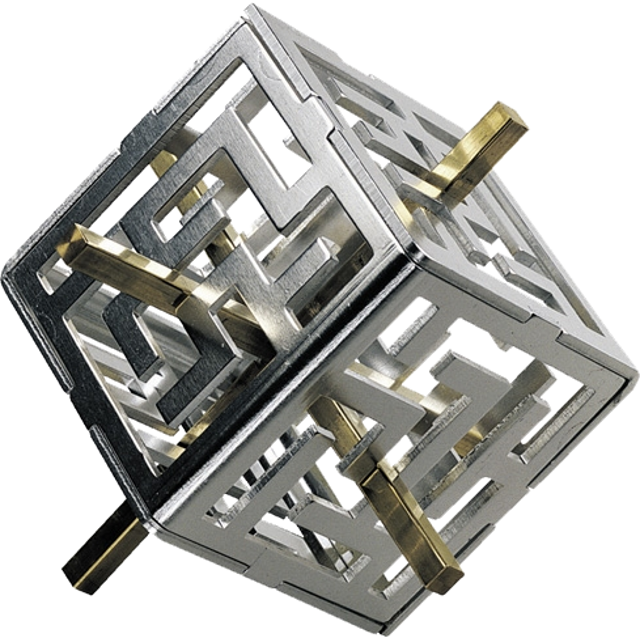
\includegraphics[width=0.6\textwidth]{images/oscar}
	\caption{Oskar's Cube (Quelle: http://www.puzzlemaster.ca)}
	\label{fig:Oskar}
\end{figure}

Die Idee eines Würfels, der die Spielwelt beschränkt, kann aus verschiedenen Gründen attraktiv sein. Die ZEISS VR-ONE ist nicht nur eine VR-Brille, sondern hat auch eine transparente Front, durch die die Handykamera aufnehmen kann. Dieses Feature soll im Konzept mit aufgenommen werden, denn es stellt einen der Unique Sellingpoints der Brille dar. Die Würfelwelt kann als Repräsentation eines Markerwürfels gesehen werden. Der Spieler hat sozusagen die Welt in der Hand und kann sie durch drehen des Markers und interner Markererkennung drehen und navigieren. 
Ein Würfel stellt durch seine sechs Seiten zudem spannende Anforderungen aber auch Freiheiten an das Art-Team bezüglich der Weltgestaltung: wie können diese interessant gestaltet werden, um den Spieler zu fesseln?
Trotzdem bietet der Würfel eine abgeschlossene Welt, was ideal für einen zeitlich stark begrenzten Game Jam ist. Die klaren Seiten bieten Orientierung für den Spieler, der durch die VR-Brille schnell diese verlieren könnte.   
  

\mysubsection{Sarah Häfele}{Erste Entscheidungen}

Die Basis ist ein großer Würfel als Spielwelt. 

Die Innenseiten des Würfels stellen Welten dar, die sich gegenüber stehen. Sie sollen durch verschiedene Rätsel, die unter anderem mit der Gravitation spielen, miteinander verbunden sein. 

Durch einen Markerwürfel soll der Spieler von außen in die Welt eingreifen und sie drehen können. Somit wird der Augmented Reality Aspekt der Brille genutzt. 

Das Ziel des Spiels könnte es sein, eine bestimmte Position zu erreichen (zum Beispiel durch ein Labyrinth den Weg finden, wie es bei Oskar's Cube der Fall ist) oder bestimmte Gegenstände einzusammeln.
   
Labyrinthe sind für ein Computerspiel, welches länger Spaß machen soll, vielleicht zu unspektakulär. Die Variante des Einsammelns kann durch verschiedene Rätsel interessant gemacht werden. Die Abhängigkeit der Seiten voneinander soll dabei jedoch trotzdem erhalten bleiben.

Eine weitere Frage wirft das Leveldesign der Welten auf: soll jede Seitenfläche des Würfels eine eigene Welt darstellen, oder soll es ein Thema für den gesamten Würfel geben. Die verschiedenen Themen können mit Rätseln verknüpft werden, weswegen die Entscheidung auf ein Thema je Seitenfläche fällt.

Die Position des Spielers ist ein weiterer wichtiger Punkt, der noch vor der groben Planung entschieden werden muss. Da das Spiel im Würfel stattfinden soll, könnte der Spieler sich entweder auf den jeweiligen Flächen bewegen, in der Mitte fest verankert sein oder sich komplett frei bewegen. Da das Thema eine gleichberechtigte Bewegung und Position erfordert, wird eine Kombination aus den oben genannten Optionen gewählt. Die Ausgangsbasis des Spielers befindet sich in der Mitte des Würfels, so dass er alle Landschaften überblicken kann. Er kann jedoch auch auf die Seiten gehen und dort die Welten erkunden.